\chapter{Sprint 3 : Gestion des tâches et Kanban}

\section*{Introduction}
Le troisième sprint constitue le cœur opérationnel de la plateforme. Il introduit
la gestion hiérarchique des tâches (avec sous-tâches), les dépendances de type
FS/SS/FF/SF avec détection de cycles (BFS), l'affectation des membres avec
allocation en pourcentage, le tableau Kanban drag-and-drop avec mise à jour
optimiste, et la saisie du temps passé.

% ============================================================
\section{Sprint Backlog}

\begin{table}[H]
  \centering
  \caption{Sprint Backlog — Sprint 3}
  \label{tab:backlog_s3}
  \begin{tabularx}{\textwidth}{C{1.2cm}L{5cm}L{2cm}C{2cm}C{1.5cm}}
    \toprule
    \thead{ID} & \thead{User Story} & \thead{Acteur} & \thead{Priorité} & \thead{Points} \\
    \midrule
    \rowcolor{lightgray}
    US-11 & Créer des tâches hiérarchiques (sous-tâches)     & Member & Must   & 8 \\
    US-12 & Définir des dépendances FS/SS/FF/SF              & Member & Must   & 8 \\
    \rowcolor{lightgray}
    US-13 & Affecter des membres avec allocation \%          & Member & Must   & 5 \\
    US-14 & Déplacer une tâche en Kanban (drag-and-drop)     & Member & Must   & 5 \\
    \rowcolor{lightgray}
    US-15 & Saisir le temps passé sur une tâche             & Member & Should & 3 \\
    US-16 & Commenter une tâche et mentionner (@)            & Member & Should & 5 \\
    \midrule
    \multicolumn{4}{r}{\textbf{Total :}} & \textbf{34} \\
    \bottomrule
  \end{tabularx}
\end{table}

% ============================================================
\section{Conception}

\subsection{Diagramme de cas d'utilisation}

\begin{figure}[H]
  \centering
  \IfFileExists{figures/sprint3_use_case.png}{%
    \includegraphics[width=0.88\textwidth]{figures/sprint3_use_case.png}%
  }{%
    \fbox{\parbox{0.88\textwidth}{\centering\vspace{1.8cm}
      \textbf{[IMAGE A INSÉRER]}\\[0.4em]
      \texttt{figures/sprint3\_use\_case.png}\\[0.3em]
      \textit{Cas d'utilisation : Member, Chef. Dépendances, détection cycle, export CSV}
    \vspace{1.8cm}}}%
  }
  \caption{Diagramme de cas d'utilisation — Sprint 3}
  \label{fig:uc_s3}
\end{figure}

\subsection{Diagramme de séquence — Déplacement Kanban}

\begin{figure}[H]
  \centering
  \IfFileExists{figures/sprint3_sequence_kanban.png}{%
    \includegraphics[width=0.90\textwidth]{figures/sprint3_sequence_kanban.png}%
  }{%
    \fbox{\parbox{0.90\textwidth}{\centering\vspace{1.8cm}
      \textbf{[IMAGE A INSÉRER]}\\[0.4em]
      \texttt{figures/sprint3\_sequence\_kanban.png}\\[0.3em]
      \textit{Séquence drag-and-drop Kanban : mise à jour optimiste → PATCH API → broadcast Reverb}
    \vspace{1.8cm}}}%
  }
  \caption{Diagramme de séquence — Déplacement d'une tâche sur le Kanban}
  \label{fig:seq_kanban}
\end{figure}

Le déplacement d'une tâche se déroule en six étapes : (1) drag-and-drop de la
carte, (2) mise à jour optimiste de l'interface React, (3) \texttt{PATCH
/api/tasks/\{id\}/move}, (4) vérification par \texttt{CheckProjectAccess}, (5)
mise à jour en base et diffusion via Laravel Reverb, (6) les autres clients
connectés reçoivent l'événement WebSocket et mettent à jour leur vue. En cas
d'erreur serveur, la mise à jour optimiste est annulée (\textit{rollback} React
Query).

\subsection{Diagramme de classes}

\begin{figure}[H]
  \centering
  \IfFileExists{figures/sprint3_class.png}{%
    \includegraphics[width=0.88\textwidth]{figures/sprint3_class.png}%
  }{%
    \fbox{\parbox{0.88\textwidth}{\centering\vspace{1.8cm}
      \textbf{[IMAGE A INSÉRER]}\\[0.4em]
      \texttt{figures/sprint3\_class.png}\\[0.3em]
      \textit{Classes : Task, TaskAssignment, TaskDependency, TaskComment, Attachment, TimeEntry}
    \vspace{1.8cm}}}%
  }
  \caption{Diagramme de classes — Sprint 3}
  \label{fig:class_s3}
\end{figure}

% ============================================================
\section{Réalisation}

\subsection{Vue Kanban}

\begin{figure}[H]
  \centering
  \IfFileExists{figures/sprint3_14_kanban.png}{%
    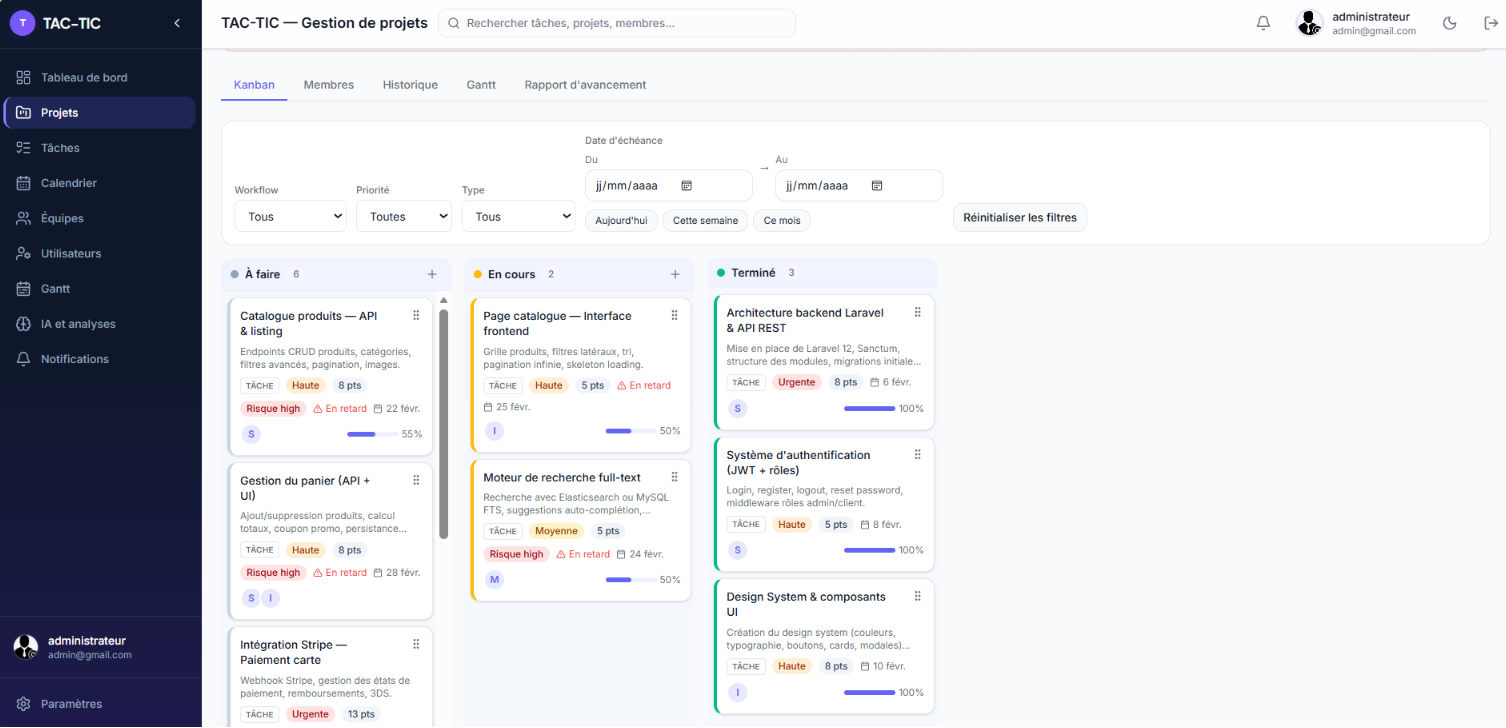
\includegraphics[width=0.90\textwidth]{figures/sprint3_14_kanban.png}%
  }{%
    \fbox{\parbox{0.90\textwidth}{\centering\vspace{2cm}
      \textbf{[IMAGE A INSÉRER]}\\[0.4em]
      \texttt{figures/sprint3\_14\_kanban.png}\\[0.3em]
      \textit{Tableau Kanban : colonnes À faire / En cours / À risque / Terminé, drag-and-drop}
    \vspace{2cm}}}%
  }
  \caption{Tableau Kanban — Drag-and-drop avec mise à jour temps réel}
  \label{fig:ui_kanban}
\end{figure}

\subsection{Formulaire wizard 4 étapes}

\begin{figure}[H]
  \centering
  \begin{subfigure}[b]{0.48\textwidth}
    \IfFileExists{figures/sprint3_15_task_step1.png}{%
      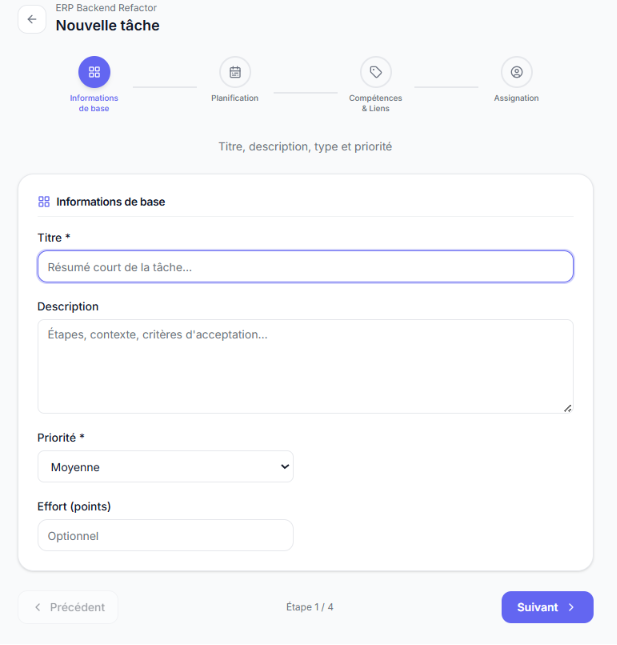
\includegraphics[width=\textwidth]{figures/sprint3_15_task_step1.png}%
    }{%
      \fbox{\parbox{\textwidth}{\centering\vspace{1.2cm}\small
        \texttt{sprint3\_15\_task\_step1.png}\\Étape 1 : Infos de base\vspace{1.2cm}}}%
    }
    \caption{Étape 1 : Infos de base}
  \end{subfigure}
  \hfill
  \begin{subfigure}[b]{0.48\textwidth}
    \IfFileExists{figures/sprint3_16_task_step2.png}{%
      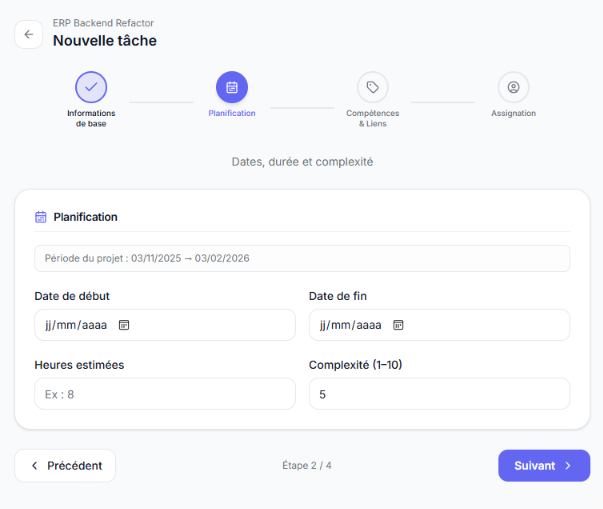
\includegraphics[width=\textwidth]{figures/sprint3_16_task_step2.png}%
    }{%
      \fbox{\parbox{\textwidth}{\centering\vspace{1.2cm}\small
        \texttt{sprint3\_16\_task\_step2.png}\\Étape 2 : Planification\vspace{1.2cm}}}%
    }
    \caption{Étape 2 : Planification et dates}
  \end{subfigure}
  \caption{Wizard de création de tâche — Étapes 1 et 2}
  \label{fig:ui_wizard_1_2}
\end{figure}

\begin{figure}[H]
  \centering
  \begin{subfigure}[b]{0.48\textwidth}
    \IfFileExists{figures/sprint3_17_task_step3.png}{%
      
\includegraphics[width=\textwidth]{figures/sprint3_17_task_step3.png}%
    }{%
      \fbox{\parbox{\textwidth}{\centering\vspace{1.2cm}\small
        \texttt{sprint3\_17\_task\_step3.png}\\Étape 3 : Dépendances\vspace{1.2cm}}}%
    }
    \caption{Étape 3 : Compétences et dépendances}
  \end{subfigure}
  \hfill
  \begin{subfigure}[b]{0.48\textwidth}
    \IfFileExists{figures/sprint3_18_task_step4_ml.png}{%
      
\includegraphics[width=\textwidth]{figures/sprint3_18_task_step4_ml.png}%
    }{%
      \fbox{\parbox{\textwidth}{\centering\vspace{1.2cm}\small
        \texttt{sprint3\_18\_task\_step4\_ml.png}\\Étape 4 : Assignation ML\vspace{1.2cm}}}%
    }
    \caption{Étape 4 : Recommandation IA}
  \end{subfigure}
  \caption{Wizard de création de tâche — Étapes 3 et 4}
  \label{fig:ui_wizard_3_4}
\end{figure}

% ============================================================
\subsection{Recherche et filtrage des tâches}

La plateforme intègre un système de recherche et filtrage multicritères permettant
à l'utilisateur de localiser rapidement une tâche parmi l'ensemble du projet.

\begin{table}[H]
  \centering
  \caption{Paramètres de recherche et filtrage des tâches}
  \label{tab:filtres_taches}
  \begin{tabularx}{\textwidth}{L{4cm}L{3.5cm}X}
    \toprule
    \thead{Filtre} & \thead{Type} & \thead{Description} \\
    \midrule
    \rowcolor{lightgray}
    Recherche textuelle  & Champ libre     & Recherche dans titre, description, commentaires \\
    Statut Kanban        & Multi-sélection & Filtrer par colonne(s) Kanban \\
    \rowcolor{lightgray}
    Priorité             & Multi-sélection & Critique / Haute / Moyenne / Basse \\
    Assigné              & Sélecteur       & Filtrer par membre assigné \\
    \rowcolor{lightgray}
    Sprint               & Sélecteur       & Sprint courant, backlog, tous \\
    Plage de dates       & Calendrier      & Date de début et/ou d'échéance \\
    \rowcolor{lightgray}
    Score de risque IA   & Curseur         & Seuil minimum de risque (0--100) \\
    Tâches en retard     & Bascule         & Afficher uniquement les tâches dépassées \\
    \bottomrule
  \end{tabularx}
\end{table}

Côté backend, la recherche est implémentée via \textbf{Eloquent scopes} chaînés :
chaque filtre actif ajoute une clause \texttt{WHERE} ou \texttt{LIKE} à la requête
SQL, optimisée par des index sur les colonnes \texttt{priority}, \texttt{status\_id}
et \texttt{due\_date}. La réponse est paginée (20 éléments par page) et mise en
cache côté client par TanStack React Query avec une durée de fraîcheur de 30\,s.

\begin{lstlisting}[style=phpstyle,caption={Scope de filtrage des tâches — TaskFilter},
  label={lst:task_filter}]
// Extrait de App\QueryFilters\TaskFilter
public function apply(Builder $query, array $filters): Builder
{
    return $query
        ->when($filters['search'] ?? null, fn($q, $v) =>
            $q->where('title', 'like', "%{$v}%")
              ->orWhere('description', 'like', "%{$v}%"))
        ->when($filters['priority'] ?? null, fn($q, $v) =>
            $q->whereIn('priority', (array) $v))
        ->when($filters['assignee_id'] ?? null, fn($q, $v) =>
            $q->whereHas('assignments', fn($s) =>
                $s->where('user_id', $v)))
        ->when($filters['overdue'] ?? false, fn($q) =>
            $q->where('due_date', '<', now())
              ->where('workflow_status', '!=', 'done'));
}
\end{lstlisting}

% ============================================================
\section{Tests unitaires}

\begin{lstlisting}[style=phpstyle,caption={Tests unitaires — Dépendances et Kanban},label={lst:tests_s3}]
it('detects direct cycle', function () {
    $task = Task::factory()->create();
    expect(fn() => app(TaskDependencyService::class)->add($task, $task->id))
        ->toThrow(HttpException::class, 422);
});

it('detects indirect cycle A -> B -> C -> A', function () {
    [$a, $b, $c] = Task::factory()->count(3)->create();
    app(TaskDependencyService::class)->add($b, $a->id);
    app(TaskDependencyService::class)->add($c, $b->id);
    expect(fn() => app(TaskDependencyService::class)->add($a, $c->id))
        ->toThrow(HttpException::class, 422);
});

it('moves task to new kanban column', function () {
    $task   = Task::factory()->create(['workflow_status' => 'todo']);
    $status = TaskStatus::factory()->create(['project_id' => $task->project_id]);
    $this->actingAs($task->project->owner)
         ->patchJson("/api/tasks/{$task->id}/move", [
             'status_id'       => $status->id,
             'workflow_status' => 'in_progress',
         ])->assertOk()
           ->assertJsonFragment(['workflow_status' => 'in_progress']);
});
\end{lstlisting}

\begin{chapconclusion}
Le sprint~3 a livré 34 story points avec une qualité élevée. Le wizard 4 étapes a
significativement amélioré la qualité de saisie : les champs obligatoires en étape~1,
les dates avec validations en étape~2, les compétences et dépendances en étape~3, et
la recommandation IA en étape~4. La détection de cycles BFS protège l'intégrité des
données. Le Kanban drag-and-drop avec mise à jour optimiste et le filtrage multicritères
sont, selon les retours utilisateurs, les fonctionnalités les plus appréciées du sprint.
\end{chapconclusion}
